\documentclass[12pt, oribibl]{extarticle}
%Some packages I commonly use.
\usepackage[english]{babel}
\usepackage{graphicx}
\usepackage{framed}
\usepackage[normalem]{ulem}
\usepackage{amsmath}
\usepackage{amsthm}
\usepackage{amssymb}
\usepackage{amsfonts}
\usepackage{enumerate}
\usepackage[utf8]{inputenc}
\usepackage[top=1 in,bottom=1in, left=1 in, right=1 in]{geometry}

\usepackage{mathtools}
\DeclarePairedDelimiter{\ceil}{\lceil}{\rceil}

%% Zitate
\usepackage[numbers]{natbib}
\bibliographystyle{abbrvnat}
%\bibliographystyle{dinat}
%\bibliographystyle{plainnat}
%\bibliographystyle{splncs}
%% Similar to option "sectionbib" but \refname instead of \bibname
\makeatletter
\renewcommand\bibsection{\section*{\refname\@mkboth{\MakeUppercase{\refname}}{\MakeUppercase{\refname}}}}
\makeatother


%A bunch of definitions that make my life easier
\setlength{\columnseprule}{1 pt}


\newtheorem{lemma}{Lemma}[section]
\newtheorem{corollary}[lemma]{Corollary}
\newtheorem{theorem}[lemma]{Theorem}
\newtheorem{definition}[lemma]{Definition}

\title{Maximum Cardinality Matching}
\author{Narek Bojikian, Piotr Witkowski, Martin Vogel}
\date{July 2019}

\begin{document}

\maketitle

\section{Introduction}
Maximum matching is a well studied optimization problem on graphs in the theory of computer science. It was first introduced through assignment problem, which is given a set of $A$ of workers and $B$ of machines of the same size and a function $f:A\times B \rightarrow \mathbb{R}^{+}$ that assigns a value of efficiency for each worker on each machine, the problem seeks an injective assignment of workers to machines such that the total efficiency is maximized.

In this report, we describe the most common ideas and approaches to solve the problem and their efficient algorithms. We presented them at the Efficient Algorithms and Data Structures Seminar at HU Berlin during summer semester 2019.

The problem has many different variations. Intuitively, in a given a graph, the goal is to pack pairs of adjacent vertices. In the weighted version of the problem we assign a weight function to each edge and try to find a packing with maximum weight. In this report we are only interested in the unweighted part, where we try to maximize the number of pairs in the packing.

\subsection{Notation}
We notate $\Delta$  to the symmetric difference of two sets, meaning for two sets $A, B$ over the same universe we define $A\Delta B := \left( A \setminus B \right) \cup \left( B \setminus A \right)$.

Some section-specific notations will be defined later in the corresponding sections.

\section{Definitions}
In this section, we formally define the problem and some necessary terms for the solution.

\begin{definition}
A \textbf{Matching} $M \subseteq E$ in a graph $G(V, E)$ is a subset of pairwise disjoint edges in the graph, meaning the edges of a matching do not overlap in their endpoints and hence no vertex can be incident to more than one edge in a matching.
\end{definition}
In a matching, a vertex incident to a matching edge is called \textbf{blocked} vertex in contrast to a \textbf{free} vertex that is not incident to a matching edge.

We say that a matching $M$ \textbf{saturates} a vertex set $S \subseteq V$, if every vertex in $S$ is incident to an edge in the matching $M$.

\begin{definition}
A \textbf{Maximal Matching} in a graph is a matching that is not a subset of any other matching in the graph, and hence a matching is maximal if and only if it intersects every single edge in the graph.
\end{definition}

\begin{definition}
A \textbf{Maximum Matching} in a graph, is a matching of the maximum cardinality in the graph. Hence any maximum matching is a maximal matching but the implication is not necessarily true in the other direction.
\end{definition}.
Note that maximum matching might not be unique in a graph. However, in this report, we will study the problem of finding any maximum matching for a given graph.

\begin{definition}
A \textbf{Perfect Matching} in a graph of $n$ vertices, where $n$ is a positive even integer, is a matching of size $n/2$.
\end{definition}
Note that since each edge is incident to two vertices and no vertex is incident to more that one matching edge, there is no matching of size greater than $\ceil*{ \frac{n}{2}}$ and hence a perfect matching *if it exists* in a graph, is a maximum matching as well.

Note also that all vertices in a perfect matching are blocked vertices and hence a perfect matching in a graph saturates the vertex set of the graph.

Perfect matching is not unique as well, and the problem of counting perfect matchings in a graph has also been well studied. We refer to [todo] for a reference.

\begin{definition}
	A Bipartite graph $G(A,B,E)$ is a graph defined on the set of vertices $A \cup B$ where $A$ and $B$ are disjoint and all edges in the graph have one endpoint in $A$ and the other in $B$, i.e. $E \subseteq A \times B$.
\end{definition}
Note that the subgraph induced by the set $A$ (or $B$) is an indipendent set in a bipartite graph.

Note that all cycles in a bipartite graph must have an even length.

Note that a bipartite graph with $|A| \neq |B|$ can not admit a perfect matching.


\clearpage

\section{Bipartite Matching}
In this section we will focus on bipartite graphs, going through some basic defintions and lemmas and describing efficient algorithms to find a maximum matching in a bipartite graph.
\begin{definition}
	A \textbf{Vertex Cover} in a graph $G(V, E)$, is a set of vertices $S \subseteq V$, such that any edge in the graph is incident to at least one vertex in the set.
\end{definition}
Minimum Vertex Cover is a well known optimization problem and it is known to be an np-hard problem \cite{karp1972reducibility}.

It is easy to see that the size of vertex cover is an aupper bound to the size of maximum matching since each edge in the matching must have an endpoint in the cover and the edges do not intersect in their endpoints. However, a very basic theorem proposed by König 1931 \cite{konig1931graphen} states that both numbers are equal in bipartite graphs. The proof is constructive that given a maximum matching in a bipartite graph we can build  a vertex cover of the same size. We omit the proof since it is technical and refer to the paper for further reading.

\begin{theorem}Koenigs Theorem

	The size of the minimum vertex cover in a graph is equal to the size of maximum matching in the graph.
\end{theorem}

In addition, Hall's theorem is another very basic theorem in bipartite graph. It describes a certificate for a graph not admitting a perfect matching and it is very essential from the algorithmic point of view.
\begin{theorem}Hall's Mariage Theorem

	Let $G(A, B, E)$ be a bipartite graph. The graph has a matching that saturates $A$, if and only if for any subset $S \subseteq A$, it holds that $|N(S)| \geq |S|$.
\end{theorem}
Using Hall's theorem, it suffices to find such a subset $S \in A$ with nieghborhood with smaller cardinality to certifiy that the graph does not admit a perfect matching.

It is easy to see why it holds in the $\impliedby$ direction, since a perfect matching can be seen as an injective map from $A$ to $B$ using the edges of the matching. It is clear that a subset $S$ with smaller neighborhood would not admit such an injective map.

The other direction can be proved by induction over the size of the set $A$. We omit the proof due to its technicalities and refer to the source for further reading \cite{hall2009representatives}.

Now we move to an algorithmic part of the problem, introducing two more definitions that we will depend on heavily in this report.

\begin{definition}
	Let $G(V, E)$ be a given graph and $M$ a fixed matching in the graph, an \textbf{Alternating Path} $P$ in relation to $M$ is a path in $G$ such that for each two consecutive edges in the path exactly one of them belongs to $M$. That means  the path goes alternatively between edges belonging to and not belonging to the matching $M$.
\end{definition}

\begin{definition}
	And \textbf{Augmenting path} in a graph $G(V, E)$ in relation to a matching $M$, is an alternating path in relation to $M$ that starts and ends in $M$-free vertices.
\end{definition}
It is easy to see, that for a matching $M$ and an $M$-augmenting path $P$, the set $M \Delta E(P)$ is a matching as well and that $|M \Delta E(P)| = |M| + 1$, and that is why it is called augmenting path.

Augmenting paths are very interesting from the algorithm point of view, since finding and augmenting path increases the size of the matching by one.

We present now Brege lemma \cite{berge1957two}, that completes our previous knowledge to a method to find maximum matching in a bipartite graph.
\begin{lemma}Berge Lemma

	Let $M, N$ be two matchings in a graph $G(V, E)$. Assume that $|N| \geq |M|$ and $|N| - |M| = k \in \mathbb{N}$, then the set $M \Delta N$ has at least $|N| - |M|$ vertex-disjoint augmenting paths in relation to $M$.
\end{lemma}
\begin{proof}
	Since each vertex can be incident to at most one edge in a matching, the graph $H(V, N \Delta M)$ has maximum degree at most $2$. Which means its connected components are simple cycles, simple paths and points. Moreover, all such paths and cycles are alternating since no two adjacent edges can correspond to the same matching. Moreover, the graph has no odd cycle since an odd cycle must have to adjacent edges from the same matching and all its even cycles and even simple paths have as many $N$ edges as $M$.

	Hence, the only components with unequal number of edges from both matchings are simple paths with odd length since the begin and end with edge from the same matching. Since $|N| - |M| = k$, there is at least $k$ odd paths in $H$ beginning and ending in $N$ edges. These paths must be $N$-augmenting paths in $G$, since they are alternating and if the endpoints were blocked in $N$, we could have extended the connected component to more edges.
\end{proof}
\begin{corollary}
	A matching $M$ in a graph $G$ is maximum, if and only if $G$ admits no $M$ augmenting paths.
\end{corollary}
\begin{proof}
If $G$ admits an augmenting path, it is ofcourse not maximum since we can compute $M \Delta P$ a greater matching in the graph.
Now assuming $M$ is not maixmum. Let us fix a maximum matching $N$. Since $|N| > |M|$, the graph $G$ admits at least $|N| - |M|$ vertex disjoint $M$-augmenting paths.
\end{proof}

Using the prvious proof, we get a method to find maximum matching in bipartite graphs. It is called the \textbf{Hungarian Method} refering to the founders of the method and it iteratively finds augmenting paths in the graph until the graph admits no more augmenting paths and hence the matching is maximum. It runs in $O(N^4)$ in a naive implementation, however we will aim in this section to a $O(\sqrt n \cdot m)$ algorithm by Hopcroft and Kapr using this exact method.

Before we go further with the Hungarian method, we would like to introduce a linear time reduction from maximum bipartite matching to max flow problem. This reduction renders any max-flow algorithm into a bipartite algorithm in the same running time. We refer to \cite{orlin2013max} for an $O(n\cdot m)$ algorithm for maximum flow problem. Using the reduction we get an algorithm for maximum matching problem in the same running time as well. 

As we shall see in the reduction, the size of the flow in the new instance is equal to the size of matching in the original instance and hence never greater than $n$. That being said, even the less efficient algorithms for maximum flow problems like Ford-Fulkerson's would give exactly the same bound for matching since $O(|f|\cdot m) = O(n \cdot m)$. Hence we can apply the reduction and use such an algorithm for maximum flow getting an $O(n \cdot m)$ algorithm for maximum matching.

\begin{reduction}
	Let $G(A, B, E)$ be a given bipartite graph for maximum matching problem. We build the instance $\left(G'(V', E', s, t), \omega\right)$ for max flow, where omega is a capacity function that assign value one to all edges of the graph $G'$, i.e. $\omega:E'\mapsto \mathbb{R}, \omega(e) = 1$ and $s$ and $t$ are two additional vertices in the graph $G'$ that play the role of the source and the sink of the matching.

	We define $V' := V \cup \{s, t\}$, and $E' := \{(a, b) : a \in A, (a, b) \in E\} \cup \{ (s, a): a \in A\} \cup \{(b, t): b \in B\}$.
	Now we claim that $G'$ with capacities $\omega$ admits a flow of size $k \geq 0$ from $s$ to $t$ if and only if the graph $G$ admits a matching of size $k$ as well.
\end{reduction}

\begin{proof}
	Let us fix a matching of size $M$ of cardinality $k$ in the graph $G$. We define a funciton $f:E'\mapsto \mathbb{R}$. We show it is a flow function and it assigns a flow of size exactly $k$.  	

	For a vertex $a \in A$, we set
	\begin{equation*}
		f((s, a)) :=
		\begin{cases}
			1& a \text{ is a blocked vertex in } M\\
			0& Otherwise\\
		\end{cases}
	\end{equation*}
	For a vertex $b \in B$, we set
	\begin{equation*}
		f((b, t)) :=
		\begin{cases}
			1& b \text{ is a blocked vertex in } M\\
			0& Otherwise\\
		\end{cases}
	\end{equation*}
	For each edge $\{a, b\} \in E$, we set
	\begin{equation*}
		f((a, b)) :=
		\begin{cases}
			1& \{a, b\} \in M\\
			0& Otherwise\\
		\end{cases}
	\end{equation*}
	It is easy to see why $f$ is a flow, since for each vertex in $V$, it has one unit input and one unit output if and only if it is blocked and hence the flow is onserved and never greater than the capacity 1.

	Now since we assign as many ones to edges coming from $s$ as there are blocked $A$ vertices, the value of the flow is $k$ as well.

	Now for a given flow function $f$ of value $k$, we build the set $M \subseteq E$, where $M := \{a, b\}, f((a,b)) = 1$. We claim $M$ is a matching of size $k$.

	Each unit of flow leaving $s$ must reach $t$ and hence use and edge in $E$ which gives the size bound.

	Now to prove it is a flow, each vertex in $A$ gets at most one unit of flow from $s$, and due to flow conservation, it can send at most one unit to $B$. For the same reason a $B$ vertex can receive at most one flow unit from $A$ and hence can be matched to at most one vertex.
\end{proof}

Now we can move to the last part of this section, namely Hopcroft and Carp's implementation\cite{hopcroft1973n} of the Hungarian method that runs in $O(\sqrt n \cdot m)$.

First we need a couple of auxiliary lemmas. We give a brief proof of the lemmas here. Please refer to the original paper for further reading.

The intuition of the algorithm is to look iteratively for shortest augmenting paths instead of arbitrary ones wich reduce the number of times we need to look for augmenting paths

A shortest augmenting path can be found using a BFS in linear time in the graph.

In addition, instead of finding one augmenting path in each iteration, we will be aiming for maximal set of vertex-disjoint shortest augmenting paths which is shortest augmenting path packing referred to by \textbf{SAPP}.

A SAPP can be found in linear time in the graph as we will describe later. We will prove that at most $2\sqrt n + 1$ such packings are enoguh to reach a maximum matching in the graph and hence in running time $O(\sqrt n \cdot m)$ we can find a maximum matching assuming the graph is connected and hence $n \notin \Omega(m)$.

We start by showing an algorithm to find a SAPP in linear time in the size of the graph. We omit the proof due to its technicalities and refer to the paper for murther readings. The proof is kinda straightforward from the algorithm.

We start with a BFS from the free vertices in $A$ building the level graph, where vertices in level $i$ have an alternating path of distance $i$ from a free vertex.

We stop our search algorithm when we reach a level with free vertex in the set $B$ after we complete building this level. Free vertices in this level are all $B$-free vertices that can be reached from $A$ free vertices using a shortes augmenting path. Hence we can build a SAPP using DFS from each such vertices using only vertices from previous level in each step until we get back to vertices in level - 0.

Note that since we are only looking for a maximal set (and not maximum), a greedy algorithm using dfs over this set of vertices suffice for our needs.

We mark each vertex as visited when we visit it the first time and hence all DFS calls can be done in $O(n + m)$ as well. 

Now we proceed with proving that $O(\sqrt n)$ rounds of SAPP are enough to find a maximum matching.

\begin{lemma}
	Let $M$ be a matching in $G$. Let $P$ be an $M$-shortest augmenting path. Let $P'$ be a shortest augmenting path in $G$ after augmenting $P$. then it holds
	\[
		|P'| \geq |P| + 2 |P \cap P'|
	\]
\end{lemma}
\begin{proof}
	Let $M' = M \Delta P$ and $M'' = M' \Delta P'$. Note that $M'' \Delta M = (M'' \Delta M') \Delta (M' \Delta M) = P' \Delta P$.

	Since $|M''| = |M| + 2$, there are two vertex disjoint augmenting paths $P_1, P_2$ in $M \Delta M''$ in relation to $M$ using Berge lemma. Since $P$ was shortest augmenting path, it holds that $|P| \leq |P_1|$ and $|P| \leq |P_2|$.

	Hence
	\begin{align*}
		|P \Delta P'|&\\
		=& |M \Delta M''|\\
		\geq& |P_1 \cup P_2|\\
		=& |P_1| + |P_2|\\
		\geq& 2 \cdot |P|\\
	\end{align*}
	Note that the inequality in the third line holds since $P_1$ and $P_2$ are in defintion part of the symmetric difference of the two matchings meanwhile the equality in the following line holds because the two paths are vertex disjoint.

	Now using this result it is easy to complete the proof.
	\begin{align*}
		&|P \Delta P'| = |P| + |P'| - 2 |P \cup P'| \geq 2 \cdot |P|\\
		\implies&|P'| \geq |P| + 2|P \cup P'|\\
	\end{align*}

	
\end{proof}


\begin{corollary}
	The length of shortest augmenting path increases monotonously in a graph after each augmentation.
\end{corollary}

Now in the following we prove that this length increases strictly after each augmenting of a SAPP.

\begin{lemma}
	Let $G$ be a given graph and $M$ a matching in $G$, Let $\mathcal{P} =  P_1, \dots P_k$ be a SAPP in the graph. Let in addtion $P$ be a shortest augmenting path in $G$ after augmenting $\mathcal{P}$. Then the length of $P$ is at least greater than $|P_1|$ the length of paths in $\mathcal{P}$.
\end{lemma}
\begin{proof}
	We distinct two cases. In the first case, assume that $P$ is disjoint from all paths in $\mathcal{P}$, if $P$ is not strictly longer that $P_1$, we could have packed it in the packing getting a greater packing and hence our packing is not maximal which is a contradiction. Hence $|P| > |P_1|$.

	For the other case let $P_i \mathcal{P}$ be a path intersecting $P$ for some $i \in [k]$. $P$ is a shortest augmenting path after augmenting paths in $\mathcal{P}$, since the length of shortest augmenting path never decrease, using the previous lemma, we know
	$$|P| \geq |P_i| + 2 |P \cap P_i|$$  
	With non empty intersection and hence the length of $P$ is strictly greater as well.
\end{proof}

Now to the final theorem of the sectoin.
\begin{theorem}
	In a graph $G$, $O(\sqrt n)$ phases of finding SAPP and augmenting them is enough to find a maixmum matching in the graph.
\end{theorem}
\begin{proof}
	Let $M$ be the matching after $\sqrt n$ phases. Using the previous lemma we know the length of the shortest augmenting path must be at least $\sqrt n + 1$. Now Let $N$ be a maximum matching in the graph. We want to bound the size oef $|N| - |M|$ and hence the number of augmenting paths we still need to find.

	Using Berge lemma, we know there is in $M$ $|N| - |M|$ vertex disjoint augmenting paths. assuming $|N| - |M| > \sqrt n$, $G$, $G$ has at least $\sqrt n$ vertex disjoint augmenting paths each of length at least $\sqrt n + 1$ which total in more than $\sqrt n * (\sqrt n + 1) > n$ vertices which is impossible. Hence $|N| - |M| \leq \sqrt n$ and hence with at most $\sqrt n$ augmenting paths we reach a maximum matching in the graph. Since each phase finds at least one augmenting path, at most $\sqrt n$ phases suffice as well. In total we have $2 \sqrt n$ phases.
\end{proof}

\clearpage

\section{Matching in General graphs}
\subsection{Edmonds' Blossom Algorithm}

The Blossom Algorithm \cite{edmonds1965paths} is an algorithm for finding maximum matching in general graphs. Given a graph $G = (V, E)$, the algorithm finds a matching $M$ such that each vertex in $V$ is incident with at most one edge in $M$ and $|M|$ is maximized.

%\vspace{1em}

\textbf{Motivation} As we learned before, bipartite graphs are a special case, where Matching problem can be efficiently solved. Unfortunately, proposed algorithms do not produce solutions (optimal solutions of the Cardinality Matching or the correct solutions of the Maximum Cardinality Matching) when applied to general graphs. Without further speculations about complexity of both general and special cases, we can pose the following question: What property of bipartite graphs is lost and cannot be utilized, when the problem is loosened to the general case?

\begin{figure}
	\centering
	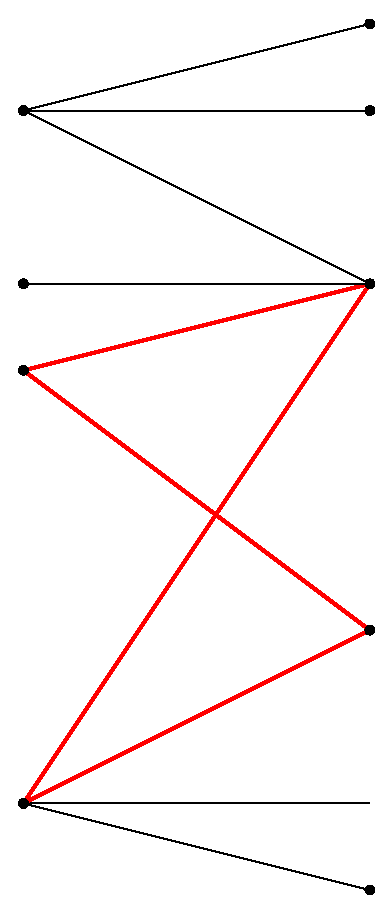
\includegraphics[height=0.4\textwidth]{img/bipartite-even-cycle.eps}
	\caption{Bipartite graphs can have cycles, but only of even length}
	\label{fig:bipartite-even-cycle}
\end{figure}

\begin{figure}
	\centering
	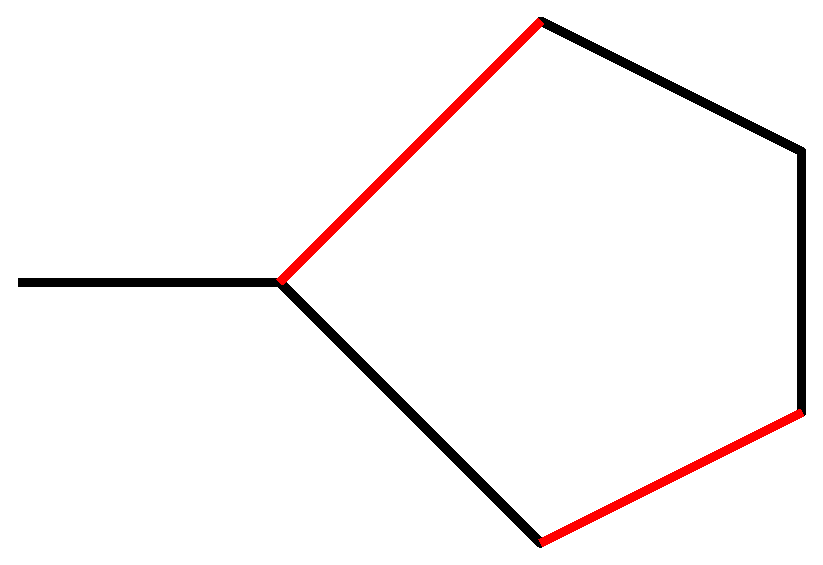
\includegraphics[height=0.2\textwidth]{img/odd-matching-maximal.eps}
	\hspace{2em}
	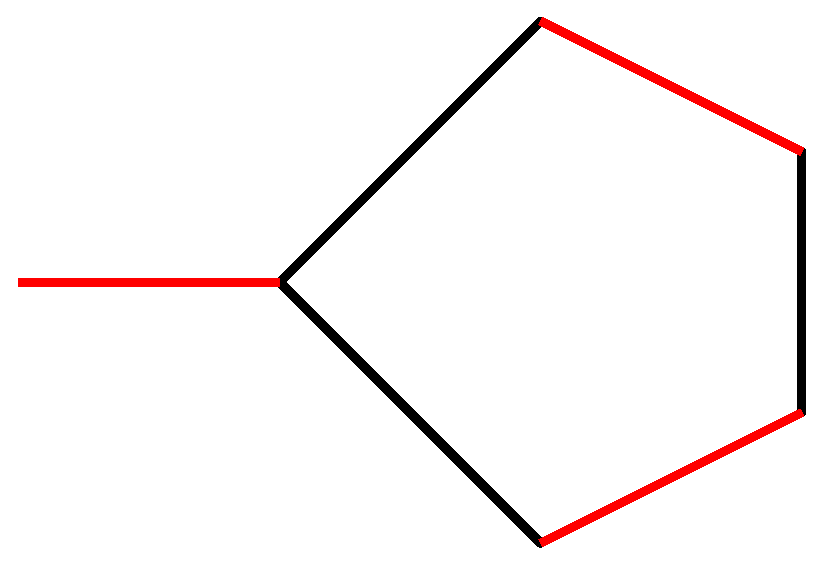
\includegraphics[height=0.2\textwidth]{img/odd-matching-optimal.eps}
	\caption{Maximal: matching of size 2, optimum: matching of size 3}
	\label{fig:maximal-optimal-cycle}
\end{figure}

\textbf{Observation} One of the benefits of having graph's edges only between two disjoint (sub)sets of vertices is that all possible cycles in the graph are of the even length (Fig. \ref{fig:bipartite-even-cycle}). If the cycle has an odd length, it is possible that (for example, greedy-generated) solutions will be sub-optimal (Fig. \ref{fig:maximal-optimal-cycle}).

Blossom algorithm uses the idea of Berge’s Theorem \cite{berge1957two}, that
matching is a maximum matching iff there is no augmenting path.
It takes Graph $G$, initial matching $M$ on $G$ as \textit{input} values and produces maximum matching $M^*$ on $G$ as \textit{output}. Starting from an initial matching, the algorithm computes a maximum matching by augmenting the current matching with augmenting paths as long as it can find them and returns whenever no augmenting paths are left. 

\textbf{Problem} How to guarantee no augmenting paths in a graph?

\begin{definition}
	\textbf{Exposed vertex} Vertex $v$ is exposed iff no edge of $M$ is incident with $v$.
\end{definition}

\begin{definition}
	\textbf{Blossom} B is a cycle in G consisting of 2k+1 edges of which exactly k belong to M, and where one of the vertices v of the cycle (base) is such that there exists an alternating path of even length (stem) from v to an exposed vertex w.
\end{definition}

\begin{definition}
	\textbf{Contracted Graph} G’ the graph obtained from G by contracting every edge of a blossom B into one vertex.
\end{definition}

\begin{figure}
	\centering
	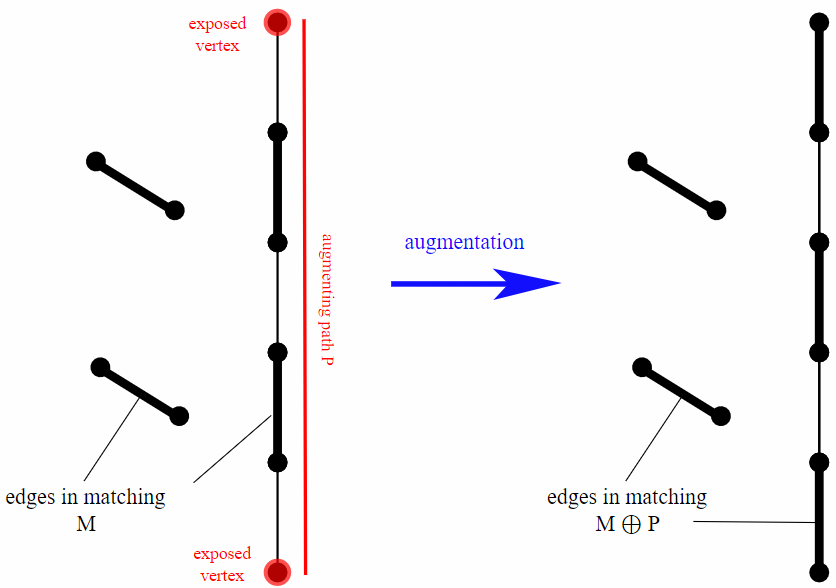
\includegraphics[width=0.75\textwidth]{img/Edmonds_augmenting_path.png}
	\caption{Augmenting a path}
	\label{fig:augmenting-a-path}
\end{figure}

\textbf{Finding an augmenting path} The search for an augmenting path uses an auxiliary data structure consisting of a forest F whose individual trees correspond to specific portions of the graph G. In fact, the forest F is the same that would be used to find maximum matchings in bipartite graphs (without need for shrinking blossoms). In each iteration the algorithm either (1) finds an augmenting path (Fig. \ref{fig:augmenting-a-path}), (2) finds a blossom and recurses onto the corresponding contracted graph, or (3) concludes there are no augmenting paths.

\textbf{Finding Blossoms}
The algorithm traverses the graph starting from an exposed vertex. Computing the set of exposed vertices can be done cheaply by substracting the vertices of $M$ from $G$. Starting from that vertex, it labels it as an outer vertex "o". Then, it alternates the labeling between vertices being inner "i" and outer "o" such that no two adjacent vertices have the same label. If two adjacent vertices are labeled as outer "o" then an odd-length cycle (and therefore a blossom) is found. See Fig. \ref{fig:contracting-a-blossom}.

\begin{figure}
	\centering
	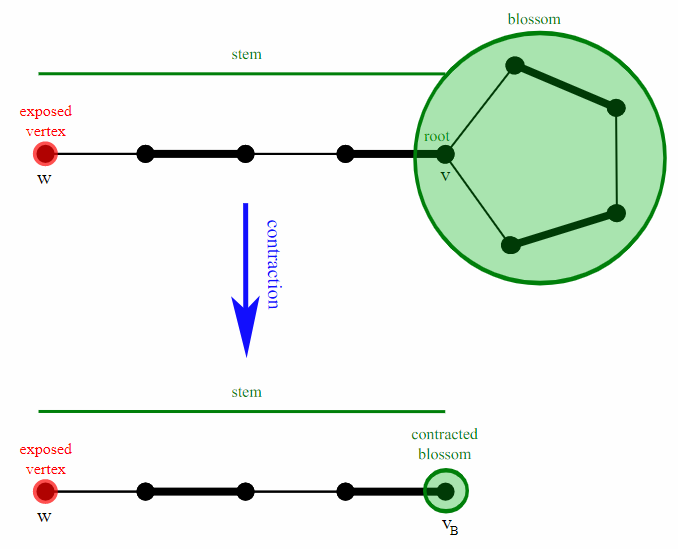
\includegraphics[width=0.75\textwidth]{img/Edmonds_blossom_contraction}
	\caption{Contracting a blossom}
	\label{fig:contracting-a-blossom}
\end{figure}

After finding and contracting a blossom, the algorithm is executed recursively on the contracted graph. For general graphs, a straightforward implementation of the maximum matching algorithm of Edmonds runs in $\mathcal{O}(|V|^4)$ time \cite{papadimitriou1982combinatorial}. However, more efficient algorithms like the one from \cite{micali1980v} which runs in
$\mathcal{O}(\sqrt{|V|}*|E|)$ are known.


\clearpage

\section{Randomized Perfect Matching Algorithm}
In this section, we describe a randomized algorithm, that efficiently checks if a given graph admits a perfect matching. In the exercises, we ask you to use this algorithm to solve the decision version of maximum matching, where given a graph $G$ and a number $k$, the problem is to find if the graph admits a maximum matching of size $k$. 

Using some exponential search algorithm, we can efficiently use an algorithm for the decision version of a problem to solve the original one and hence we get an efficient randomized algorithm for maximum matching in general graphs.

Actually we will only present the bipartite case in this section. Using some tricks to deal with odd cycles (skew symmetric matrices) the solution can be extended to the general case.

We start by recalling some basics from linear algebra and mathematics.
\begin{definition}
A function $f:A \mapsto B$ is a \textbf{Bijection}, iff for any elements $b \in B$ there is exactly one elements $a \in A$ such that $a \mapsto b$.
\end{definition}
Note that $A$ and $B$ must be of the same cardinality in order to define a bijection between them.

\begin{definition}
	A \textbf{Permutation} $\pi(S)$ over a set $S$ is a bijection from $S$ to itself.
\end{definition}
We denote the set of all permutations over a set $S$ by $\mathcal{S}_S$.

We denote the set of all permutations over the set $[n]$ for $n \in \mathbb{N}$ by $\mathcal{S}_n$.

\begin{definition}
	For a given bipartite graph $G(A, B, E)$ where $|A| = |B| = n \in \mathbb{N}$, let $a_1, \dots, a_n$ be some enumeration for the vertices in $A$. Similarly, let $b_1, \dots, b_n$ be an enumeration for the vertices in $B$.
	
	We define the \textbf{Bipartite Matrix} $A_G$ of the graph $G$ as $A_G := \left\{a_{i, j}\right\}_{n \times n}$, where 
	\begin{equation*}
		a_{i,j} =
		\begin{cases}
			1, & \{a_i, b_j\} \in E\\
			0, & Otherwise\\
		\end{cases}
	\end{equation*}
\end{definition}

In addition we recall the terms \textbf{Determinant} and \textbf{Permanent} of a matrix.
Formally, The Determinant of a matrix $A := \{a_{i, j}\}_{n \times n} \in \mathbb{R}^{n \times n}$ is given by the formula
\[
	det(A) = \sum\limits_{\pi \in \mathcal{S}_n} \left( sign(\pi) \prod\limits_{i \in [n]} a_{i, \pi(i)}  \right)
\]
Where $sign(\pi)$ of a permutation $\pi$ is defined as following.
Let $r$ be the number of swaps needed to turn a permutation to into identity function. Where a swap in a permutation is a new permutation $\pi'$ such that we fix two elements $i$ and $j$, and set $\pi'(k) := \pi(k)$ for all $k \notin \{i, j\}$, $\pi'(i) = \pi(j)$ and $\pi'(j) := \pi(i)$.
Then we can define $sign$ as follow
	\begin{equation*}
		a_{i,j} =
		\begin{cases}
			1, & r \equiv 0 mod 2\\
			-1, & Otherwise\\
		\end{cases}
	\end{equation*}
Even though the value of $r$ is not unique. It is easy to see that its parity is always unique which makes $sign$ function well defined.

On the other hand we define a permanent of a matrix as follow
\[
	perm(A) = \sum\limits_{\pi \in \mathcal{S}_n} \left( \prod\limits_{i \in [n]} a_{i, \pi(i)}  \right)
\]

Even though permanent and determinant are very similar in their definitions, determinant of a matrix can be found in slightly super quadratic time \cite{aho1974design}, meanwhile finding the permanent of a matrix is a hard problem \cite{valiant1979complexity} and probably does not admit a polynomial algorithm.

Now we begin with the main part of the section. Let $G(A, B, E)$ be a given graph. Let $a_1, \dots, a_n$ be an arbitrary enumeration of elements in $A$ and $b_1, \dots, b_n$ an arbitrary enumeration of elements in $B$. In addition, let $A_G$ be the bipartite matrix of $G$ according to the previous enumerations. 

Assume the given graph admits a perfect matching, each vertex in $A$ is matched to a vertex in $B$. The function $f$ assigning each vertex to each matched vertex defines a permutation $\pi$ where $\pi(i) = j$ for $f(a_i) = b_j$.

It is easy now to see that a graph admits a perfect matching if and only if there is a permutation $pi$, for which the edge $\{i, \pi(i)\}$ is a part of the graph and hence $a_{i, \pi(i)} = 1$.

Formally speaking, we are looking for a permutation $\pi$ such that
\[
	\prod\limits_{i \in [n]} a_{i, \pi(i)} = 1
\]
Let us call such a permutation \textbf{good}.

However, since any such product is either one or zero, we can write the previous condition as
\[
	\sum\limits_{\pi \in \mathcal{S}_n}\left( \prod\limits_{i \in [n]} a_{i, \pi(i)}\right) \neq 0
\]

Now comparing this formula to the  formula of permanent, it is clear that a graph admits a perfect matching if and only if the permanent of its bipartite graph is non zero.

Note that this formula computes a stronger results. It is equal to the number of perfect matchings in a graph. However, as stated above, finding a permanent of a matrix is a hard problem and hence not probably computable in polynomial time.

We might try to use the determinant of a matrix instead. However, it might occur that we have exactly as many good permutations with positive $sign$ as good permutations with negative $sign$ which will cancel out in the previous formula.

In order to overcome this problem, we first note that we do not have to restrict our selves to the value one in the bipartite matrix. Since we are only interested in non-zero products, we can turn the ones into any non-zero real value and good permutation will still have non zero product while not good ones will have product zero.

More interestingly, we can use variables instead of values, defining the matrix $A'_G = \{a'_{i,j}\}_{n\times n}$ for a graph $G(A, B, E)$, where
	\begin{equation*}
		a'_{i,j} =
		\begin{cases}
			x_{i,j}, & \{a_i, b_j\} \in E\\
			0, & Otherwise\\
		\end{cases}
	\end{equation*}
	where $x_{i, j}$ is some variable over some field $\mathcal{F}$. Note that the determinant of this matrix is now a polynomial of degree $n$.
	
	We prove the following lemma.
	\begin{lemma}
		A bipartite graph $G(V, E)$ admits a perfect matching if and only if the determinant of the matrix $A'_G$ is not the identical zero.
	\end{lemma}
	\begin{proof}
		$\implies$: Let $\pi$ be the good permutation defining this perfect matching as defined above, i.e. $\pi(i) = j$ for $a_i$ matched to $b_j$. We substitute $1$ to each $x_{i, \pi(i)}$ and zeroes else where. This permutation will have the only non-zero product and hence the determinant will be either one or minus one according to the sign of the permutation. Since there is a values assignment for which the determinant is non-zero, it can not be identical zero.

		$\impliedby$: if the determinant is not identical zero, there is a value assignment for $x_{i, j}$, such that the determinant is not zero. Let us fix such an assignment. Now since the determinant is not zero, it can not be the case that all permutations are bad and the existence of a good permutation implies the existence of a perfect matching in the graph. 
	\end{proof}

	Now we turned the problem of checking if a bipartite admits a perfect matching into the problem of finding if a polynomial is identical zero or not. The problem here is that we cannot write this polynomial explicitly since it will require us to apply the formula above and dealing with exponentially many factors. Hence, we will be using the determinant as a black box, where we substitute values to the variables and then compute the determinant in polynomial times. This reminds us of \textbf{Schwartz Zippel} lemma.


	\begin{lemma}
		Schwartz-Zippel

		Let $\mathcal{F}$ be some field. Let $\rho$ be some polynomial of degree $d$ and $n$ variables over $\mathcal{F}$. Moreover, let $S \subseteq F^{n}$ be some subset of assignments to $\rho$, then for $(r_1 \dots r_n) \underset{u.a.r}{\in}S$. Assuming $\rho$ is not identical zero, we have
		$$Pr\left[\rho(r_1, \dots, r_n) = 0\right] \leq \frac{d}{|S|}$$
		Where we mean with $u.a.r$ that the assignment is chosen uniformly at random from $S$.
	\end{lemma}
	The lemma can easily be proven by showing that $S$ can not have more than $d |S|^{n-1}$ zeros by induction over $n$. However, we omit the proof here and refer to the original proof by Schwartz \cite{schwartz1979probabilistic}.

	Now using the previous lemma, we know the determinant has degree at most $n$, and hence choosing $F$ to be $\{0, 1\}$ and setting building the set $S$ of size $2d$ arbitrarily. We choose some random substitution from $x$. If the determinant is non-zero, we already know for sure that the graph admits a perfect matching. If the determinant is zero we know with probability one half that the graph admits no matching.

	Repeating the previous algorithm $t$ times and getting zeros every time yields that the graph admits no perfect matching with probability at least $1 - (\frac{1}{2})^t$ and hence for $d(n)$ the time needed to compute determinant of an $n$ by $n$ matrix, with $5 \log n$ repetitions we get an algorithm running in $O(d(n) \log n)$ that either outputs no if the graph admits no perfect matching or with probability at least $1 - frac{1}{n^5}$ answers yes if it admits one.

	Now as notated previously \cite{aho1974design}, determinants can be computed in sub cubic time, namely in  $O(n^\omega)$ where $\omega$ is the matrix multiplication exponent (the time needed the multiply two matrices) and the best known bound is around 2.3.

	Hence we have proved an $O(n^{\omega} \log(n))$ randomized algorithm to check if a given graph admits a perfect matching with high probability which is better than the best known $O(n^{5/2})$ deterministic algorithm by \cite{micali1980v} in dense matrices.


\bibliography{bibliography}




\end{document}
